\documentclass[titlepage]{article}

\usepackage[margin=1.0in]{geometry}

% Line numbers
%\usepackage{lineno}
%\linenumbers

% Figures
\usepackage{graphicx}
\graphicspath{{figures/}}

% Trick Latex into placing all figures and tables at the end of the document
% regardless of their position in the source code.
\renewcommand{\textfraction}{1.0}
\renewcommand{\floatpagefraction}{0.9}

% Equations
\usepackage{amsmath}

% Bibliography
\usepackage{natbib}

% Better tables
\usepackage{booktabs}
\usepackage{multirow}
\newcommand{\ra}[1]{\renewcommand{\arraystretch}{#1}}

% Headers
\usepackage{fancyhdr}
\pagestyle{fancy}
\lhead{Team MechE}
\rhead{Cloud Droplet Growth}
\renewcommand{\headrulewidth}{0.4pt}


%--------------------------------------------------
% TITLE
%--------------------------------------------------
\title{SIO 217A: Cloud Droplet Growth}
\author{Team MecheE \\ Bengu Ozge Akyurek, David Larson, Guangchao Wang}
\date{\today}

\begin{document}

\maketitle


%--------------------------------------------------
% INTRO
%--------------------------------------------------
\section{Introduction}
Atmospheric thermodynamics focuses on water and its transformations. Advanced
topics are usually focused on phase transitions of water, homogeneous and
heterogeneous nucleation, and the role of supersaturation on the formation of ice
crystals and cloud droplets. Among those sub-topics, cloud nucleation has been
a large area of research throughout the twentieth century.

Nucleation process is an energy balance between surface tension and
latent heat. When the latent heat associated with condensation is enough to
counteract the surface tension on the drop, the droplet is nucleated. However, the
surface tension of a small water droplet can be very large. In order to break
the high energy barrier on the surface for homegeneous nucleation, high values
of supersaturation ($>>$ 100\%) are required.

In the Earth's atmosphere supersaturation typically only slightly exceeds
100\%, e.g., 100.05\%.  Therefore cloud droplets are formed via hetereogeneous
nucleation, which involes cloud condensation nuclei (CCN), a subset of aerosol
particles. The presence of CCN, such as sodium chloride (NaCl), lower the
equilibrium vapor pressure of the water relative to pure water, thereby
reducing the effects of surface tension and enabling the formation of cloud
droplets.

In this study we evaluate the effects of CCN on droplet growth within warm
clouds, which form due to vapor-to-liquid condensation. Water droplets are
assumed to be isolated and spherical, and form due to the diffusion of
water vapor to the surface in a steady state diffusion field.


%--------------------------------------------------
% MODEL
%--------------------------------------------------
\section{Cloud Droplet Growth}

\subsection{Model Description}
In order to model the cloud droplet growth as a function of time, we have used
Equation~\eqref{eq:5.26} from \cite{Curry}.  The approximation assumes that a
droplet has the shape of a sphere that develops around a saturated nucleus
core. Furthermore, the environment conditions (temperature, pressure, and
supersaturation) are assumed to be constant, and the solute and curvature
effects are neglected, which will be explained in more detail. The initial
approximation is obtained by applying diffusion equations to the droplet, as
shown in Equation~\eqref{eq:Diffusion}.

\begin{equation}
    \label{eq:Diffusion}
    \dfrac{dm}{dt}=4 \pi r D_{v} \left( \rho_{v}(\infty) - \rho_{v}(r) \right)
\end{equation}

Adding the latent heat by condensation, shown in
Equation~\eqref{eq:LatentHeat}, gives the basis of the droplet growth rate
model.

\begin{equation}
    \label{eq:LatentHeat}
    \dfrac{dQ}{dt}=-L_{lv}\dfrac{dm}{dt}=-4 \pi r \kappa \left( T(\infty) - T(r) \right)
\end{equation}

These equations are combined to approximate the growth rate of a droplet by
diffusion as
\begin{align}
    \label{eq:5.26}
    r \frac{dr}{dt} = (S - 1) \left[ \frac{L_{lv}^2 \rho_l}{\kappa R_v T^2} + \frac{\rho_l R_v T}{e_s(T) D_v} \right] ^{-1} = \frac{S - 1}{K + D}
\end{align}
where $K$ and $D$ are the thermodynamic terms associated with heat conduction
and diffusion of water vapor, respectively. This differential equation is the
same as Equation 5.26 in \cite{Mason}. $S$ is the saturation ratio, $\rho_l$
the liquid density, $e_s$ the saturation pressure in the droplet and $T$ is the
environment temperature.

Assuming the atmospheric ambient conditions are constant (i.e. $T$, $S$, $K$,
and $D$ are constant), then Equation~\eqref{eq:5.26} can be integrated to get
\begin{align}
    \label{eq:5.27}
    r(t) = \left[ r_0^2 + \frac{2(S -1)}{K + D}(t - t_0) \right] ^{1/2},
\end{align}
which can then be rearranged to find $t$

\begin{align}
    \label{eq:5.27T}
    t = (r^2 - r_0^2) \frac{K + D}{2(S - 1)}
\end{align}

Using the values from Table~\ref{tab:parameters}, the main results in
Table~\ref{tab:Table5.5} can be approximated. But to include the effects of
initial mass, curvature and the solute, we must modify our model.


\begin{table}[h]
    \centering
    \caption{Parameters for droplet growth rate.}
    \label{tab:parameters}

    \begin{tabular}{l l l l}
    \toprule
    Parameter & Value & Units & Notes\\
    \midrule
    $S - 1$   & 0.05            & \%                         & \\
    $p$       & 900             & $mb$                       & \\
    $T$       & 273             & $K$                        & \\
    $r_0$     & 0.75            & $\mu m$                    & \\
    $L_{lv}$  & 2.5x10$^{6}$    & $J \ kg^{-1}$              & pure water at $T=273 K$ \\
    $\rho_l$  & 1000            & $kg \ m^{-3}$              & pure water at $T=273 K$ \\
    $R_v$     & 461             & $J \ kg^{-1} K^{-1}$       & \\
    $\kappa$  & 2.4x10$^{-2}$   & $J \ m^{-1} s^{-1} K^{-1}$ & $T=273 K$ \\
    $D_v$     & 2.21x10$^{-5}$  & $m^2 s^{-1}$               & $T=273 K$, $p=1000 mb$ \\
              & 2.46x10$^{-5}$  & $m^2 s^{-1}$               & $T=273 K$, $p=900 mb$ \\
    $e_s (T)$ & 6.15            & $mb$                       & $T=273 K$\\
    \bottomrule
    \end{tabular}
\end{table}


\begin{table}[h]
    \centering
    \caption{Growth rate of droplets with nuclei of NaCl, ($S - 1$)=0.05\%,
        $p$=900mb, $T$=273K, and $r_0$=0.75$\mu$m recreated from Table 5.5 of \cite{Curry}.}
    \label{tab:Table5.5}

    \ra{1.2}
    \begin{tabular}{@{} c r r r @{}}
        \\
        \toprule
        m [g] & $10^{-14}$ & $10^{-13}$ & $10^{-12}$ \\
        \midrule
        r [$\mu$m] & \multicolumn{3}{c}{t [s]} \\
        \midrule
        1  & 2.4    & 0.15   & 0.013 \\
        2  & 130    & 7.0    & 0.61 \\
        4  & 1,000  & 320    & 62 \\
        10 & 2,700  & 1,800  & 870 \\
        20 & 8,500  & 7,400  & 5,900 \\
        30 & 17,500 & 16,000 & 14,500 \\
        50 & 44,500 & 43,500 & 41,500 \\
        \bottomrule
    \end{tabular}
\end{table}


One of the main properties of Equation~\eqref{eq:5.27T} is that it does not
depend on the nucleus mass, which directly contradicts with
Table~\ref{tab:Table5.5}. This led us to the first modification on the
approximation Equation~\eqref{eq:5.27T}. Rather than starting from
$r=r_{0}=0.75\ 10^{-6} \mu m$ and $t_{0}=0$ as given in the conditions of
Table~\ref{tab:Table5.5}, we have altered the definition of the starting radius
as the radius of the nucleus without any water. We haven't changed the value of
$r_{0}$, as this was given as one of the constants. But, we have defined
$t_{0}$ as the time the radius of the droplet develops to $r_{0}$, which is
definitely not $0$.

To calculate the initial radius, we have assumed that the nucleus is a perfect
sphere. Thus, the initial radius can calculated as

\begin{equation}
    \label{eq:InitialRadius}
    \rho_{NaCl}\frac{4}{3}\pi r_{i}^{3}=m_{NaCl} .
\end{equation}

We have used $\rho_{NaCl}$=2160 kg m$^{-3}$. This adjustment introduced an
effect of the nucleus mass and decreased the overall error of the first given
approximation.

The secondary improvement was on $e_{s}$. The approximation assumed $e_{s}$ to
be a constant, but normally it is not. Especially for small $r$ values,
\cite{Best} states that $e_{s}$ deviates from its average value significantly.
Since our starting point involves small values of $r$, we have applied two
modifications on $e_{s}$. The first adjustment is the usage of Raoult's law to
incorporate the effect of surface tension, introducing an additional factor
depending on both $r$ and the mass of the nucleus. This factor is shown in
Equation~\eqref{eq:RaoultsLaw}. $i$ is a constant depending on the molecular
structure of the nucleus core and $i=2$ for NaCl. $e_{s\infty}$ is the
saturation pressure of the environment (at a virtual radius of $r=\infty$).

\begin{equation}
    \label{eq:RaoultsLaw}
    \dfrac{e_{s}}{e_{s\infty}} = \dfrac{n_{H2O}}{i n_{solt}+n_{H2O}} = \dfrac{\dfrac{4}{3}\pi r^{3} \rho_{H2O}}{M_{H2O}} \left[ i \dfrac{m_{solt}}{M_{solt}} + \dfrac{\dfrac{4}{3}\pi r^{3} \rho_{H2O}}{M_{H2O}} \right]
\end{equation}

The second modification is the introduction of the effect of curvature:

\begin{equation}
    \label{eq:Curvature}
    \dfrac{e_{s}}{e_{s\infty}}=\exp \left( \dfrac{2\sigma_{lv}}{\rho_{l}R_{v}Tr} \right) .
\end{equation}

The combined effect of surface tension and the curvature is then

\begin{equation}
    \label{eq:EsDefinition}
    e_{s}(r,T) = e_{s\infty} \left[ \dfrac{\dfrac{4}{3}\pi r^{3} \rho_{H2O}}{M_{H2O}} \right] \left[ i \dfrac{m_{solt}}{M_{solt}} + \dfrac{\dfrac{4}{3}\pi r^{3} \rho_{H2O}}{M_{H2O}} \right] ^{-1} \exp \left( \dfrac{2\sigma_{lv}}{\rho_{l}R_{v}Tr} \right)
\end{equation}

Throughout our calculations and simulations, we assume $T$ to be constant as
its deviations from its initial value is negligible. This modification in
$e_{s}$ directly affects our $D$ value in Equation~\eqref{eq:5.26}.


A final modification has been applied on the numerator $(S-1)$ of
Equation~\eqref{eq:5.26} as recommended by \cite{Mason}. By adding the
curvature effects we find

\begin{equation}
    \label{eq:Numerator}
    (S-1) \rightarrow (S-1)+\dfrac{2\sigma_{lv}}{\rho_{l}R_{v}Tr}-\dfrac{i n_{solt}}{i n_{solt}+n_{H2O}}
\end{equation}
where $n$ represents the mole number of the material in the subscript.


Although this equation increases the accuracy of the results, it depends itself
on $r$. This means that the simple quadratic solution in
Equation~\eqref{eq:5.27T} can not be used any more and we need a numerical
integration method to solve the differential equation in
Equation~\eqref{eq:5.26}. Using the explicit Euler method we are able to
calculate $r$ iteratively as

\begin{equation}
    \label{eq:Iteration}
    r_{k+1}= \left[ \dfrac{S - 1+\dfrac{2\sigma_{lv}}{\rho_{l}R_{v}Tr} - \dfrac{n_{solt}}{i n_{solt}+n_{H2O}}}{K(T) + D(r_{k},T)} \right] \dfrac{\Delta t}{r_{k}}
\end{equation}

The initial condition at $k=0$ is $r=r_0$ which was calculated as the radius
of the nucleus core itself.

Although this approximation is close to the values in Table~\ref{tab:Table5.5},
it has its drawbacks with respect to reality. The first limitation is that we
have assumed the temperature to be constant throughout the droplet and same as
the environment at all times. The second drawback is that we have assumed that
the environment properties like $\kappa, D_{v}, L_{lv}$ stay constant, which
introduces an extra error into our approximation.


\subsection{Model Parameters}
$K$ is the thermodynamic term related to the latent heat release due to
condensation and diffusion of heat away from the droplet.  $D$ is the vapor
diffusion term related to the diffusion of water vapor onto the growing
droplet. Plus, $S$ is saturation ratio. If $S < 1$, then $dr/ dt < 0$, which
describes the evaporation of a cloud drop. And if $S > 1$, then $dr/dt > 0$ and
the droplet grows by condensation.

Water vapor is transferred to the drop by molecular diffusion as long as the
vapor pressure surrounding the drop exceeds the saturation vapor pressure of
the drop. As water condenses on the drop, latent heat release, the drop becomes
warmer than the environment, and heat is diffused away from the drop.
Condensation can thus be considered as a double diffusive process, with water
vapor diffused towards the drop and heat diffused away from the drop. Therefore
cloud droplet growth is a balance between diffusion of water vapor and
convection.



%--------------------------------------------------
% RESULTS
%--------------------------------------------------
\section{Results of Modeling Study}
Figure~\ref{fig:r_t} shows a visual comparison between the droplet growth rate
modeled by Equation~\eqref{eq:5.27} with $r_0 = 0.75 \mu m$, $T=273 K$, $p=900
mb$, and $(S - 1) = 0.05\%$. A major assumption of Equation~\eqref{eq:5.27} is
that the curvature and solute effects are neglible once the droplet grows
beyond a few microns. The figure shows general agreement between the model and
values from Table 5.5 of \cite{Curry}. But by considering curvature and solute
effects, Equation~\eqref{eq:Iteration} is able to recreate the values from
Table 5.5 of \cite{Curry} (see Figure~\ref{fig:r_t_modified}).

\begin{figure}[h]
    \centering
    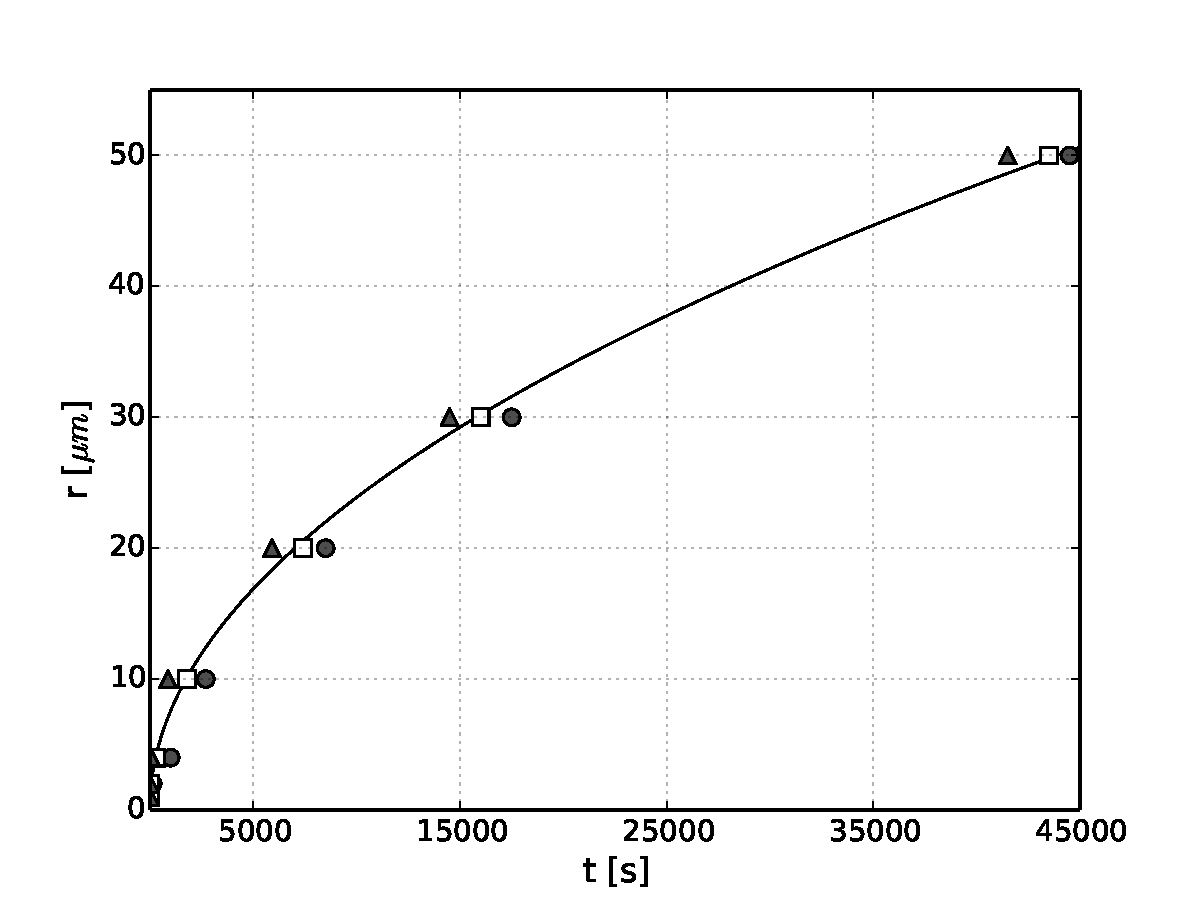
\includegraphics[width=\textwidth]{r_t.pdf}
    \caption{Droplet growth rate of the simplified model (Equation~\eqref{eq:5.27}) against the values from Table 5.5 of \cite{Curry}.}
    \label{fig:r_t}
\end{figure}

\begin{figure}[h]
    \centering
    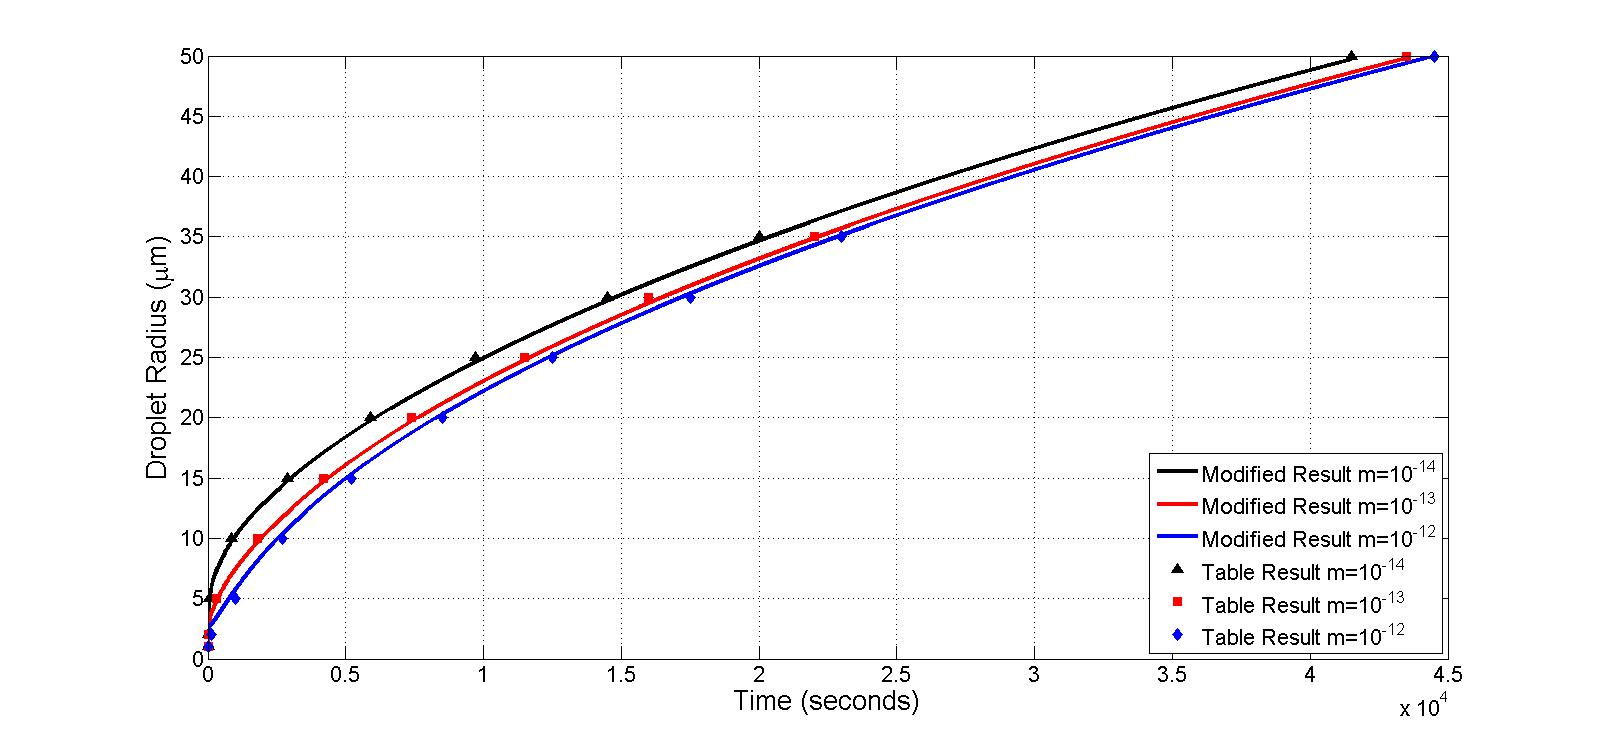
\includegraphics[width=\textwidth]{r_t_modified.jpg}
    \caption{Droplet growth rate with a nuclei of NaCl, and curvature and solute effects are included. The values are calculated numerically using Equation~\eqref{eq:Iteration} with $\Delta t = 0.1$, $T = 273 K$, $p = 900 mb$, and $S - 1 = 0.05 \%$.}
    \label{fig:r_t_modified}
\end{figure}


To study the sensitivity of the model, we varied $T$ and $(S - 1)$, separately,
while holding all other parameters constant. Figure~\ref{fig:temperature} and
~\ref{fig:supersaturation} show the results. The increased values of $T$
correspond physically to increasing the heat diffused away from the droplet
(decreased $K$) and decreasing the amount of water vapor diffused into the
droplet (increased $D$).  Similarily, increased values of $S - 1$ increase the
droplet growth rate due to an increased amount of water vapor, which lowers the
amount of energy needed to achieve activation.

\begin{figure}
    \centering
    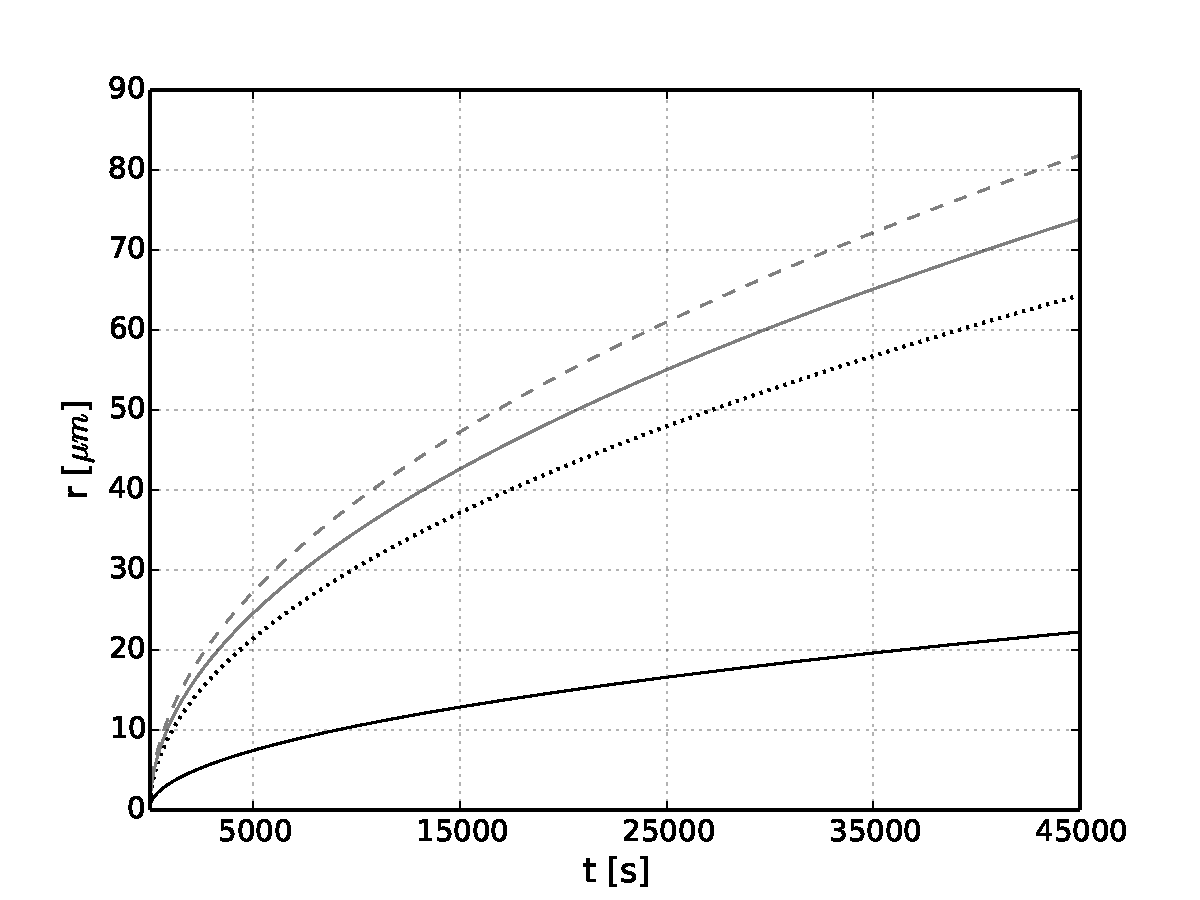
\includegraphics[width=\textwidth]{r_t_temperature.pdf}
    \caption{Droplet growth rate at $p=900 mb$ and $S - 1 = 0.05\%$ as $T$ is increased.}
    \label{fig:temperature}
\end{figure}


\begin{figure}
    \centering
    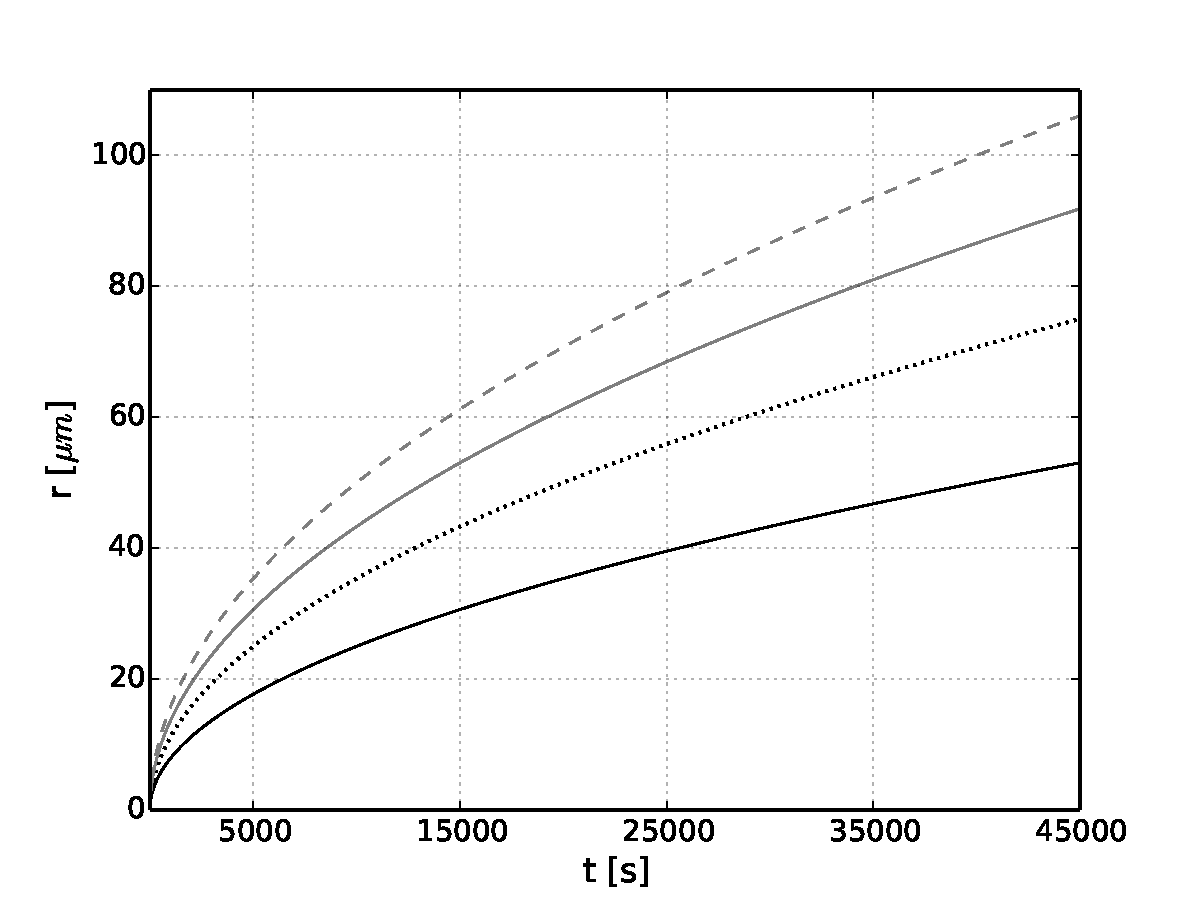
\includegraphics[width=\textwidth]{r_t_supersaturation.pdf}
    \caption{Droplet growth rate at $p=900 mb$ and $T= 273 K$ as the $S - 1$ is increased.}
    \label{fig:supersaturation}
\end{figure}


%--------------------------------------------------
% CONCLUSION
%--------------------------------------------------
\section{Conclusion}
We have evaluated two droplet growth models for clouds that form due to
vapor-to-liquid condensation. The first model, taken from \cite{Curry}, is a
simplified model that ignores curvature and solute effects, but captures the
general behavior of the droplet growth. The second model includes curvature and
solute effects, and is able to recreate the values from Table 5.5 of
\cite{Curry}. A sensitivity analysis shows a positive correlation between droplet
growth, and both temperature and supersaturation.

Both models describe droplet growth by diffusion only and therefore do not take into
account the effect of collisions and coalescence between droplets, which become
important once $r > 20 \mu m$. Additionally, the models do not consider changes
in $S$ over time as less water vapor is available. A more robust version of the
models should incorporate the effects of both coalesence and changing $S$.


%--------------------------------------------------
% BIBLIOGRAPHY
%--------------------------------------------------
\bibliography{sources}
\bibliographystyle{plainnat}


\end{document}
